\section{分子動力学(MD)シミュレーション}

分子動力学シミュレーションにより、$\beta_2$ARのinactive状態active状態双方で1000psトラジェクトリを計10本取得した。

\subsubsection{$\beta_2$ARの活性化による構造変化}
アゴニストが結合した$\beta_2$ARは、顕著な構造変化を引き起こす\cite{rasmussen2011crystal}\cite{poudel2021activation}ことがわかっている。
%参考文献:β2ARの構造変化
%2011「β2アドレナリン受容体-Gsタンパク質複合体の結晶構造」
%https://www.nature.com/articles/nature10361
%参考文献:β2ARの構造変化
%2021「β2アドレナリン受容体の活性化によるエネルギー輸送ネットワークの再編成」
%https://pubs.acs.org/doi/full/10.1021/acs.jpcb.1c03412
主な変化として以下が挙げられる:
\begin{enumerate}
    \item \textbf{TM6の外側への動き}: TM6の細胞質側末端が、約14Å外側に移動する。
    \item \textbf{TM5の外側への動き}: TM5の細胞質側末端が、外側に移動する。
    \item \textbf{TM7の内側への動き}: TM7の細胞質側末端が、内側に移動する。
\end{enumerate}

本研究で得られた、シミュレーション中の原子の平均的な配置を示した$\beta_2$ARのinactive構造とactive構造を重ね合わせたのが以下の図である。
%inactiveとactiveの重ね合わせ
\begin{figure}[htbp]
  \centering
  \begin{subfigure}{0.88\textwidth} % 各図の幅を調整
    \centering
    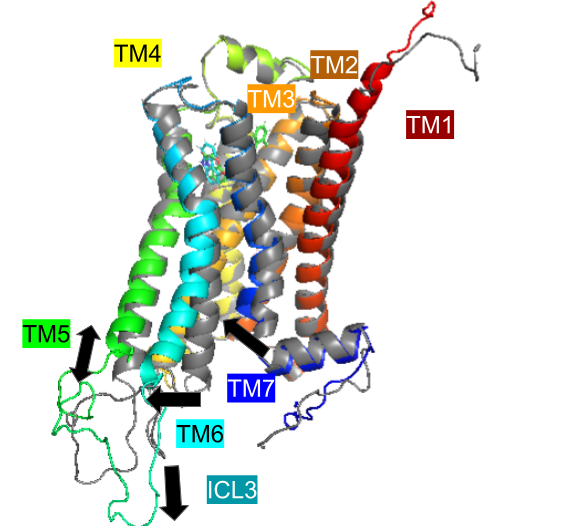
\includegraphics[width=\textwidth]{system-all-with-label.png}
    \caption{$\beta_2$ARのTM5,TM6,TM7の変化。}
    \label{fig:fitting_TM}
  \end{subfigure}
  \hspace{0.02\textwidth} % 図の間のスペース
  \begin{subfigure}{0.88\textwidth}
    \centering
    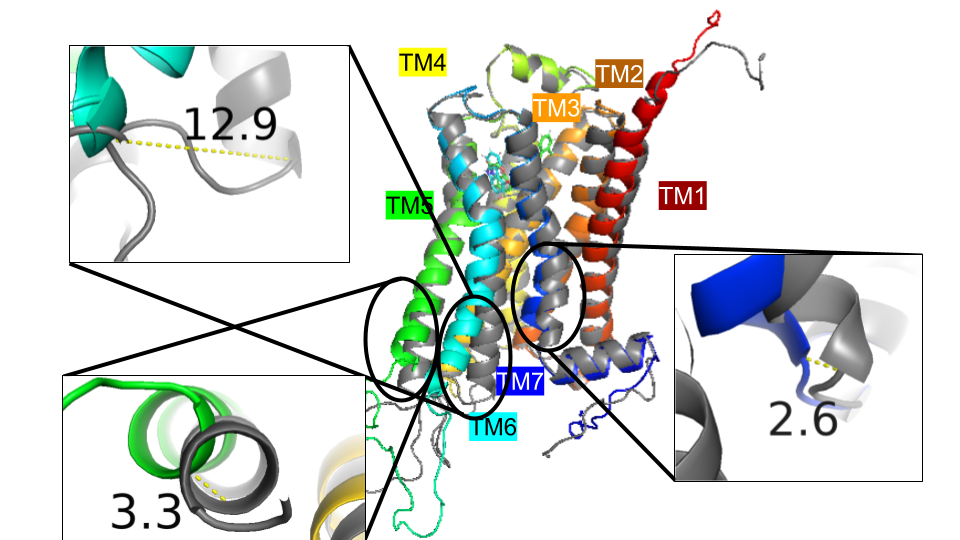
\includegraphics[width=\textwidth]{system-all-with-label-detail.png}
    \caption{$\beta_2$ARのTM5,TM6,TM7の変化の詳細。}
    \label{fig:fitting_TM_detail}
  \end{subfigure}
  \caption{$\beta_2$ARのinactive構造(灰色)とactive構造(色付き)の重ね合わせ。}
  \label{fig:fitting-all}
\end{figure}

\newpage

TM6の細胞質側末端にある残基の$\mathrm{C}_\alpha$原子が、TM7から離れる方向に12.9Å移動する様子が観察された。
TM5の細胞質側末端部分は末端の$\mathrm{C}_\alpha$原子がTM3から離れる方向に3.3Å移動する様子が観察された。
TM7の細胞質側末端にある残基の$\mathrm{C}_\alpha$原子が、タンパク質の内側に近づく方向に2.6Å移動する様子が観察された。
TM5とTM6を結ぶ細胞内ループ3(ICL3)においても、Gタンパク質結合部位を開くように特定の方向に並んでいるような様子が観察された。
シミュレーションによる活性状態と不活性状態の平均構造の違いは、先行研究で指摘されている重要な構造変化を忠実にとらえていた。

\subsubsection{$\beta_2$ARの保存された結晶水}
DOWSERによって検出された、エネルギー的に安定な水分子は、inactive状態で14869個、active状態で18876個同定された。
そのうち、シミュレーション中で保存されている結晶水はinactive状態で7個、active状態で6個同定された。

\begin{figure}[htbp]
    \centering
    \begin{subfigure}{0.48\textwidth} % 各図の幅を調整
      \centering
      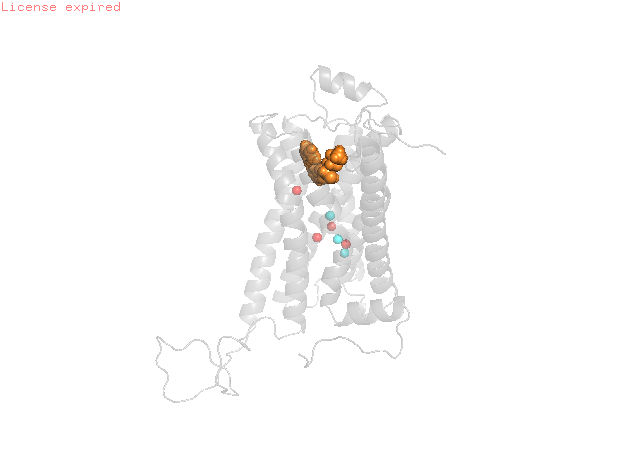
\includegraphics[width=\textwidth]{inactive_saved_water_with_saved.png}
      \caption{$\beta_2$ARのinactive状態における保存された結晶水。計7個同定され、そのうち赤で示されているのは、activeと共通で見つかった4個の水である。}
      \label{fig:inactive_water}
    \end{subfigure}
    \hspace{0.02\textwidth} % 図の間のスペース
    \begin{subfigure}{0.48\textwidth}
      \centering
      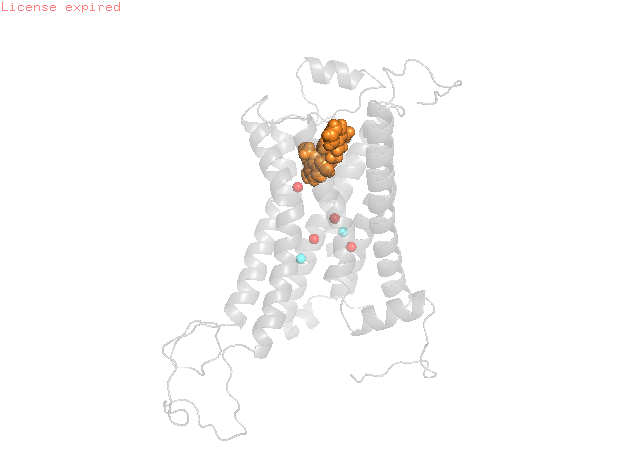
\includegraphics[width=\textwidth]{active_saved_water_with_saved.png}
      \caption{$\beta_2$ARのactive状態における保存された結晶水。計6個同定され、そのうち赤で示されているのは、inactiveと共通で見つかった4個の水である。}
      \label{fig:active_water}
    \end{subfigure}
    \caption{保存された結晶水}
    \label{fig:water-all}
  \end{figure}

\newpage

%inactiveとactiveで保存されている結晶水
重要な水分子をアミノ酸と同等のノードとして扱うため、これらの水を拡張「残基」として残基番号を振り分けた。
シミュレーション中で保存されているinactive状態の7個の結晶水、active状態の6個の結晶水のうち、
双方で共通の位置に存在していた結晶水は4つあったため、残基番号をそれぞれ(344,346,347,348)と定めた。
それ以外の結晶水は、(355,356,357,358,359)の残基番号を振り分けた。

\begin{figure}[htbp]
  \centering
  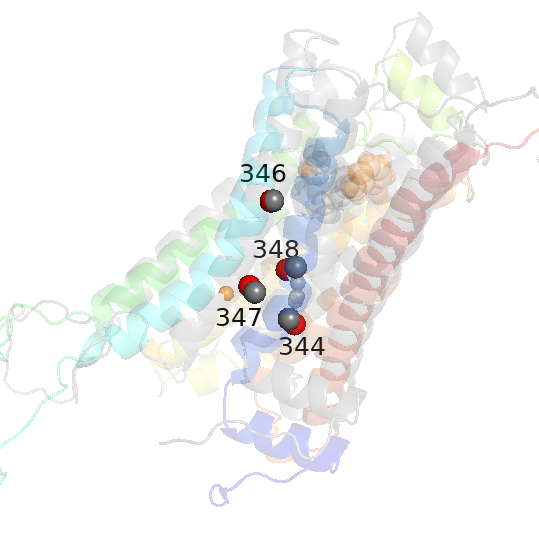
\includegraphics[width=0.8\textwidth]{xwater_fitting.png}
  \caption{保存された結晶水のうち、$\beta_2$ARのinactive状態とactive状態の双方で共通の位置に存在する水分子。}
  \label{fig:xwater_fitting}
\end{figure}

\newpage

%水分子、先行研究との比較

\section{$\beta_2$ARのinactiveおよびactive状態のコミュニティ検出}

各トラジェクトリーから得られた平均構造の座標データを基に、ネットワークのエッジの重みとして用いる残基間最短距離の2乗逆数の平均$\langle \frac{1}{d^2} \rangle$ を計算した。

エッジを以下の条件で形成させた後、エッジの重みを加え、inactive状態active状態双方のネットワークを構築した。
1. 残基ペア間の最短距離が3\,\text{\AA}未満である場合、エッジを形成する。
2. アミノ酸配列上で隣接する残基感のエッジは削除する。

以下が構築されたネットワークの詳細である。
\begin{table}[!ht]
    \centering
    \caption{ネットワーク上のノード数と、残基ペア間の最短距離が3\,\text{\AA}未満のエッジ数}
    \begin{tabular}{lll}
      \hline
      モデル名          & ノード数  & エッジ数 \\
      \hline 
      inactive(2RH1)  &  350 &  16296 \\ 
      active(3P0G)    &  349 &  15433 \\ 
    \end{tabular}
    \label{tab:network_size}
  \end{table}

構築されたネットワークを基に、コミュニティ検出を行った。
\subsubsection{Louvain法の信頼性}

ネットワークにおけるコミュニティ構造を検出するために用いたLouvain法の結果の信頼性は、モジュラリティ$Q$の値を用いて評価される。
モジュラリティ$Q$の値は通常-1から1の範囲を取り、以下のように解釈される:

\begin{itemize}
    \item \( Q \) が負:分割がネットワーク構造と一致しておらず、不適切な分割である。
    \item \( Q \) が 0 に近い:ネットワークがランダム構造に近い。
    \item \( Q \) が正:ネットワーク内にコミュニティ構造が存在する。
\end{itemize}

本研究の解析対象である$\beta_2$ARのinactiveおよびactive状態のコミュニティ検出におけるモジュラリティ$Q$の最良値および標準偏差を計算した。

\paragraph{試行回数100回におけるモジュラリティ値の平均および標準偏差}
\begin{itemize}
    \item inactive状態: \( Q = 0.5194 \pm 0.0060 \)
    \item active状態: \( Q = 0.5239 \pm 0.0006 \)
\end{itemize}
さらに、モジュラリティ値の標準誤差は以下の通りです:
\begin{itemize}
    \item inactive状態: \( \pm 0.0005 \)
    \item active状態: \( \pm 0.0004 \)
\end{itemize}

inactive状態とactive状態のモジュラリティ値はどちらも正の値を示しており、ネットワーク内に明確に分割されたコミュニティ構造があることを示唆している。

\subsection{Louvain法で検出されたコミュニティ}

以下に$\beta_2$ARのinactive構造とactive構造で検出されたコミュニティを示す。

\begin{figure}[htbp]
    \centering
    \begin{subfigure}{0.60\textwidth} % 各図の幅を調整
      \centering
      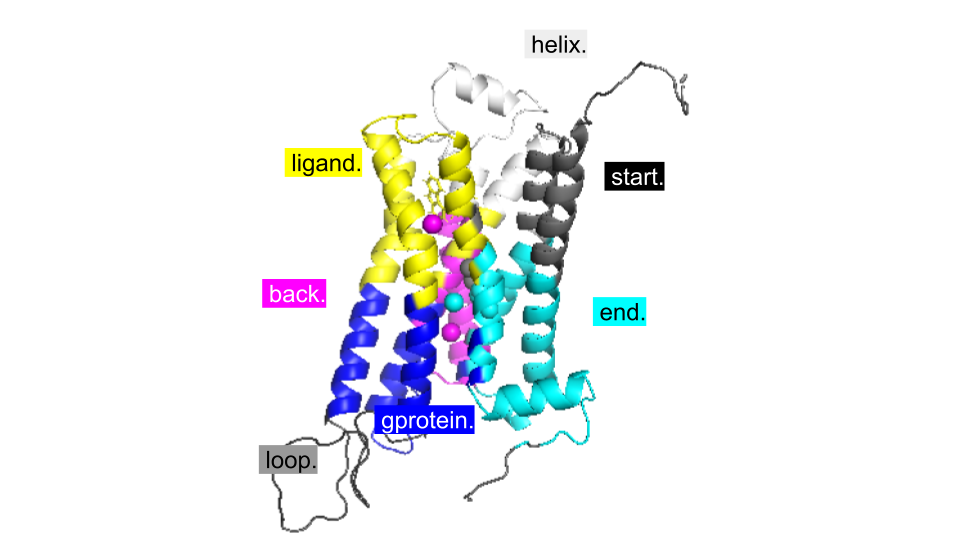
\includegraphics[width=\textwidth]{inactive_with_label.png}
      \caption{inactive状態において検出されたコミュニティ構造を色分けして示した図。各色と名付けたコミュニティは以下に表す:黒(start)、シアン(end)、白(helix)、ピンク(back)、グレー(loop)、黄色(ligand)、青(gprotein)。}
      \label{fig:inactive_community}
    \end{subfigure}
    \hspace{0.02\textwidth} % 図の間のスペース
    \begin{subfigure}{0.60\textwidth}
      \centering
      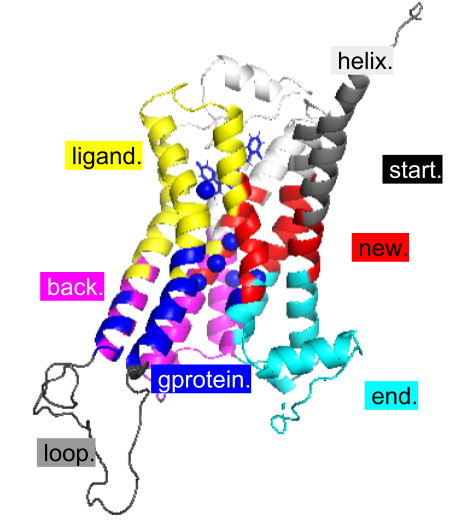
\includegraphics[width=\textwidth]{active_with_label.png}
      \caption{active状態において検出されたコミュニティ構造を色分けして示した図。各色と名付けたコミュニティは以下に表す:黒(start)、シアン(end)、白(helix)、ピンク(back)、グレー(loop)、黄色(ligand)、青(gprotein)、赤(new)。}
      \label{fig:active_community}
    \end{subfigure}
    \caption{$\beta_2$ARのLouvain法で検出されたコミュニティ構造}
    \label{fig:community-all}
  \end{figure}

\newpage

まず双方のコミュニティに共通することとして、リガンド結合部位と活性部位であるGタンパク質結合部位に対応する独立したコミュニティが、黄色(ligand)、青(gprotein)として検出された。
またinactive状態からactive状態への変化として、青(gprotein)コミュニティの再編成が起きていることと、赤(new)コミュニティが新規に形成されたことが挙げられる。

\begin{table}[!ht]
  \centering
  \caption{活性化に伴うコミュニティの再編成と、コミュニティを構成している残基群の比較}
  \resizebox{\textwidth}{!}{
    \begin{tabular}{lll}
      \hline
      活性化に伴うコミュニティの再編成  & inactiveでの構成要素  & activeでの構成要素 \\
      \hline 
      青(gprotein)コミュニティの再編成  &  TM3,TM5,TM6の細胞質側残基  &  TM6の細胞質側残基、リガンド、6つの保存された結晶水 \\
      赤(new)コミュニティの新規形成  &  なし  & TM7,TM1,TM2の中間付近に位置する残基 \\ 
    \end{tabular}
  }
  \label{tab:community_change}
\end{table}

青(gprotein)コミュニティの再編成が起きたのは、
TM5,TM6の細胞質側がタンパク質の中心から離れるように外側に動いたことで、
もともと同じ青(gprotein)コミュニティに所属していたTM3と別のコミュニティに分かれたためだと考えられる。
実際にTM6の顕著な動きにより、TM5とTM6が協調して動くことが確認されている。
%https://pubs.acs.org/doi/full/10.1021/jp506579a
しかしその独立したTM6の青(gprotein)コミュニティに、active状態に存在している保存された結晶水6つ全てとリガンドが含まれたことは興味深い結果であり、
これと、赤(new)コミュニティの新規形成が、シグナル伝達経路にどう影響を与えるかは以後の分析で考察していくこととする。
%コミュニティが1つ増えることに言及はしているが、コミュニティの解析はしていない
%https://pubs.acs.org/doi/full/10.1021/jp506579a

ここで、inactive状態とactive状態で示されているネットワークの全体密度を計算する。
全体エッジ密度$D_{\text{global}}$の計算式は以下のように表される。

\begin{equation}
  D_{\text{global}} = \frac{\sum_{i=1}^{N} \sum_{j=i+1}^{N} w(i, j)}{\tilde{\omega} \times N(N-1)}
\end{equation}

ここで
$\sum_{i=1}^{N} \sum_{j=i+1}^{N} w(i, j)$はネットワーク内の全てのエッジ重みの総和、
$\tilde{\omega}$はネットワーク全体のエッジの平均重み(全エッジの重みの総和÷全エッジ数)、
$N$はネットワーク内の全ノード数、
$N(N-1)$は理論的に存在しうるグラフ(完全グラフ)での最大エッジ数
を示している。

分子はネットワーク内の実際のエッジ重みの総和を表しており、
分母はネットワーク内の理論的に考えられる全エッジが、ネットワークの平均的な重みを持つと仮定した時に期待される重みの総和
を表している。

この式に基づいて、inactive構造とactive構造のネットワークの全体エッジ密度を計算すると、それぞれ以下のようになる。
\begin{itemize}
    \item inactive状態:\( D = 0.133 \)
    \item active状態:\( D = :0.127 \)
\end{itemize}

active状態ではネットワーク全体の密度が微減した。

\subsection{コミュニティ内およびコミュニティ間のエッジ密度}
active状態で再編成されたコミュニティや新しく検出されたコミュニティの役割を定量的に分析するために、ネットワークの全体密度$D_{\text{global}}$の計算で用いた密度の概念を用いたさらなる計算を行った。
続いて、inactive状態とactive状態双方においてそれぞれコミュニティ内のエッジ密度、コミュニティ間のエッジ密度を計算した。

\subsubsection{コミュニティ内エッジ密度}
コミュニティ内エッジ密度$D_{\text{internal}}$の計算式は以下のように表される。

まずコミュニティごとにサブグラフを作成する。
ただしコミュニティ間のエッジは削除し、独立したコミュニティを表現している。
続いてコミュニティ内エッジ密度を計算する。

\begin{equation}
  D_{\text{internal}} = \frac{\sum_{(u,v) \in E_C} w_{uv}}{\tilde{\omega} \cdot n_c (n_c - 1)}
  \label{eq:internal_density}
  \end{equation}

ここで$E_C$はコミュニティ$C$内の全エッジの集合、
$w_{uv}$はコミュニティ$C$内のノード$u$とノード$v$の間の実際のエッジ重み、
$\tilde{\omega}$はネットワーク全体のエッジの平均重み(全エッジの重みの総和÷全エッジ数)、
$n_c$はコミュニティ$C$内の全ノード数、
$n_c (n_c - 1)$は理論的に存在しうるコミュニティ内のグラフ(完全グラフ)での最大エッジ数

分子はコミュニティ内の実際のエッジ重みの総和を表しており、
分母はコミュニティ内の理論的に考えられる全エッジが、ネットワークの平均的な重みを持つと仮定した時に期待される重みの総和
を表している。

コミュニティ内エッジ密度$D_{\text{internal}}$の値は以下のように解釈される:
\begin{itemize}
    \item \( D_{\text{internal}} \) が 0 に近い:コミュニティ内のノード間での接続が少ないか、エッジの重みが非常に小さい。相互作用が弱く、コミュニティとしての結束が薄い。
    \item \( D_{\text{internal}} \) が 1 に近い:コミュニティ内のノード間の接続が非常に密であり、実際のエッジ重みが最大理論値に近い。コミュニティ内の相互作用が非常に強い。
\end{itemize}

上記の式に基づいて、inactive構造とactive構造のコミュニティ内エッジ密度を計算すると、それぞれ以下のようになる。

\begin{figure}[htbp]
    \centering
    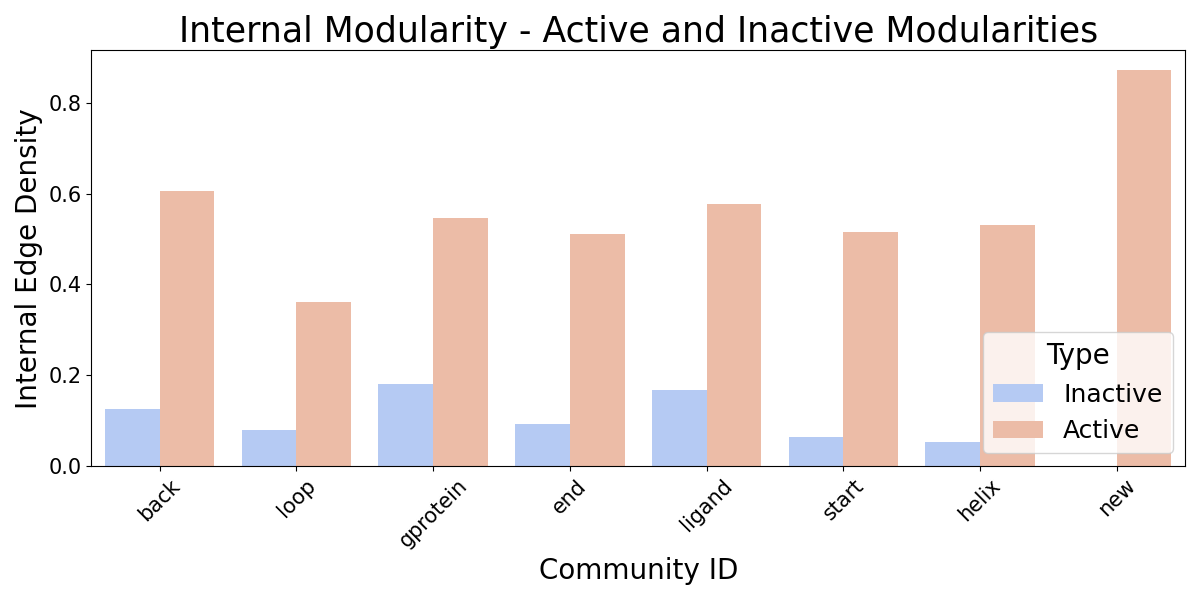
\includegraphics[width=1.0\textwidth]{internal_modularities.png}
    \caption{$\beta_2$ARのinactive状態とactive状態において検出されたコミュニティのコミュニティ内エッジ密度を示した図。コミュニティの名称は、コミュニティ構造で名付けたものである。}
    \label{fig:internal}
\end{figure}

\newpage

inactive構造では、全てのコミュニティ内エッジ密度が、0.2より低い値を示した。
しかしactive構造で全てのコミュニティのコミュニティ内エッジ密度が増加し、新たに出現したnewコミュニティは0.87という高い値を示した。
活性化に伴って、すべてのコミュニティの内部の相互作用が強い結びつきを形成している構造に変化したことがわかる。

\subsubsection{コミュニティ間エッジ密度}
コミュニティ間エッジ密度$D_{\text{inter}}$の計算式は以下のように表される。

\begin{equation}
D_{\text{inter}} = \frac{\sum_{\substack{u \in C_i \\ v \in C_j}} w_{uv}}{\tilde{\omega} \cdot n_c n_{c'}}
\label{eq:inter_density}
\end{equation}


ここで$C_i$と$C_j$は異なるコミュニティ$i$と$j$、
$w_{uv}$はコミュニティ$C_i$内のノード$u$とコミュニティ$C_j$内のノード$v$の間の実際のエッジ重み、
$\tilde{\omega}$はネットワーク全体のエッジの平均重み(全エッジの重みの総和÷全エッジ数)、
$n_c$と$n_{c'}$はコミュニティ$C_i$内とコミュニティ$C_j$内の全ノード数、
$n_c n_{c'}$は理論的に存在しうるコミュニティ$C_i$と$C_j$間のグラフ(完全グラフ)での最大エッジ数

分子はコミュニティ間の実際のエッジ重みの総和を表しており、
分母はコミュニティ間の理論的に考えられる全エッジが、ネットワークの平均的な重みを持つと仮定した時に期待される重みの総和
を表している。

コミュニティ内エッジ密度$D_{\text{inter}}$の値は以下のように解釈される:
\begin{itemize}
    \item \( D_{\text{inter}} \) が 0 に近い:異なるコミュニティ間の接続がほとんどなく、エッジの重みが小さい。コミュニティ間での相互作用がほぼ存在しないか非常に弱い。
    \item \( D_{\text{inter}} \) が 1 に近い:異なるコミュニティ間の接続が非常に密であり、実際のエッジ重みが理論値に近い。異なるコミュニティ間で強い相互作用や影響のやりとりが行われている。
\end{itemize}


上記の式に基づいて、inactive構造とactive構造のコミュニティ間エッジ密度を計算すると、それぞれ以下のようになる。

\begin{figure}[htbp]
    \centering
    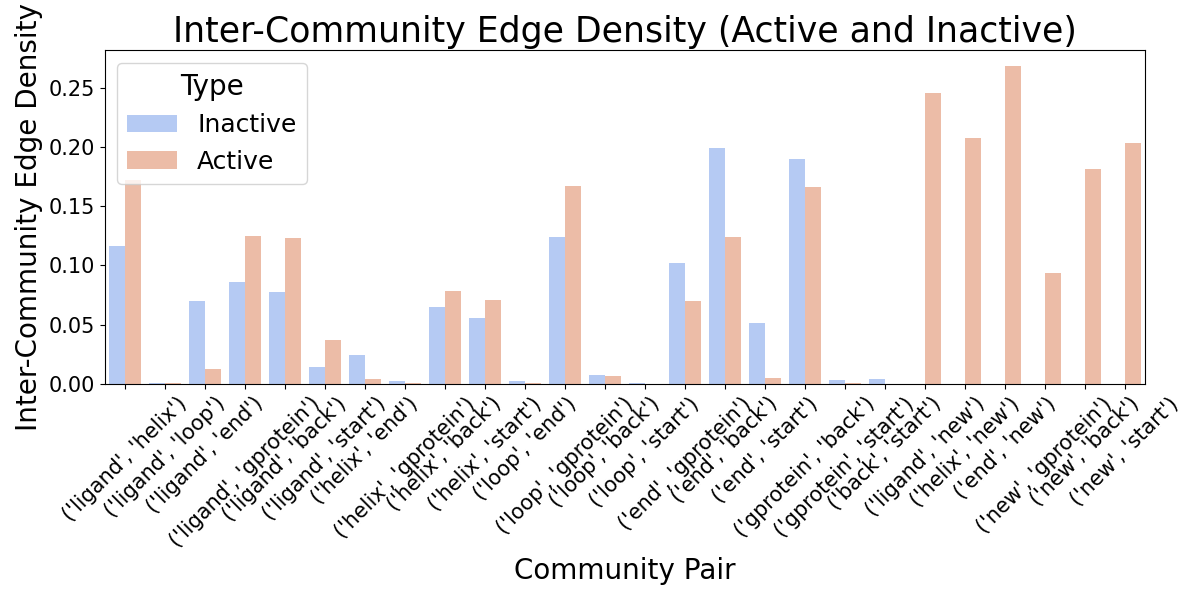
\includegraphics[width=1.0\textwidth]{interedge_modularities.png}
    \caption{$\beta_2$ARのinactive状態とactive状態において検出されたコミュニティのコミュニティ間エッジ密度を示した図。コミュニティの名称は、コミュニティ構造で名付けたものである。}
    \label{fig:inter}
\end{figure}

\newpage

ただし、inactive状態とactive状態の双方でコミュニティ間エッジ密度が0だったコミュニティペアは、図から除外している。

コミュニティ間エッジ密度$Q$の値は以下のように解釈される:
\begin{itemize}
    \item \( Q \) が 0 に近い:コミュニティ間でエッジが少なく、各コミュニティがほぼ独立している。
    \item \( Q \) が 1 に近い:コミュニティ間で多数のエッジが存在し、コミュニティ間の結びつきが強い。
\end{itemize}

active状態になると(gprotein,loop)(gprotein,ligand)(helix,ligand)(back,ligand)といったコミュニティペアが増加し、
newに関わる5つのコミュニティペアが相対的に高い値を示した。


\subsubsection{inactive状態とactive状態の全体密度、コミュニティ密度の考察}

\paragraph{密度に関わる3つの変数における、inactive状態からactive状態への変化}

ここまでinactive状態とactive状態の全体エッジ密度、コミュニティ内エッジ密度、コミュニティ間エッジ密度の変化を通じて、コミュニティ内およびコミュニティ間の相互作用を定量的に評価してきた。
\begin{enumerate}
  \item \textbf{全体エッジ密度の微減}: active状態への遷移に伴い、ネットワーク全体のエッジ密度がわずかに減少した。
\end{enumerate}

全体エッジ密度が微減したのは、TM6の12.9Åの外側への動きが影響していると考えられる。
活性化によってTM6の565個のエッジが消去されたことが以下の図でわかっている。
そこで仮にactiveのエッジ数に、TM6の外側の動き分減少したエッジ565個が追加されることになったとしたら、全体エッジ密度はどうなるかを見積もる。

\begin{equation}
  D_{\text{global}} = \frac{\sum_{i=1}^{N} \sum_{j=i+1}^{N} w(i, j)}{\tilde{\omega} \times N(N-1)}
\end{equation}

理論的に存在しうるグラフ(完全グラフ)での最大エッジ数である$N(N-1)$は変わらず、
\begin{equation}
  N(N-1) = 349(349-1) = 121602
\end{equation}
ネットワーク内の全てのエッジ重みの総和である$\sum_{i=1}^{N} \sum_{j=i+1}^{N} w(i, j)$は、
追加するエッジ565個は、全てinactiveの平均重みである2.38を重みとしてもつと仮定すると、
\begin{equation}
  \tilde{\omega} = 37,731.84+565 \times 2.38 = 39076.54
\end{equation}
ネットワーク全体のエッジの平均重み(全エッジの重みの総和÷全エッジ数)である$\tilde{\omega}$は全エッジの重みの総和を全エッジ数で割ったものになるので、
\begin{equation}
  \tilde{\omega} = \frac{39076.54}{15433+565} = 2.44
\end{equation}
最終的に全体エッジ密度は$D_{\text{global}}$は、
\begin{equation}
  D_{\text{global}} = \frac{39076.54}{2.44 \times 121602} \approx 0.132
\end{equation}
つまりinactive状態の全体エッジ密度である0.133と近い値が得られたため、
active状態で全体エッジ密度が微減したのはTM6の外側への動きによるエッジの減少が影響していると結論付けられる。


\begin{figure}[htbp]
  \centering
  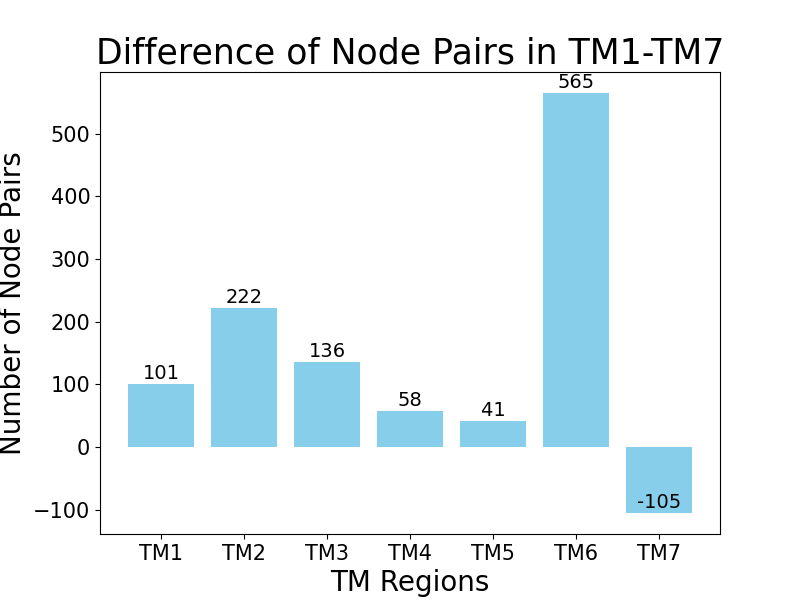
\includegraphics[width=1.0\textwidth]{added_removed_edges.png}
  \caption{$\beta_2$ARのinactive状態からactive状態におけるエッジの数の変化(消去されたエッジから加えられたエッジの数を引いたもの)を、ヘリックスごとに示した図。}
  \label{fig:inter}
\end{figure}

\newpage


\begin{enumerate}
  \item \textbf{コミュニティ内エッジ密度の増加}: active状態では、すべてのコミュニティ内エッジ密度が増加し、特にnewコミュニティが高い値を示した。
  \item \textbf{コミュニティ間エッジ密度の増加}: active状態において、ligandやgproteinに関わるコミュニティペアは増加した。新しく生成されたnewコミュニティに関連するコミュニティペアは高い値を示した。
\end{enumerate}

これらの結果は、active状態への遷移に伴う分子全体のネットワーク再編成が、
コミュニティ内部の相互作用を強化させるとともに、
情報伝達に関わる分子間の情報伝達の効率化を支える重要なメカニズムであることを示している。
特に、newコミュニティが形成されたことで、リガンド結合部位と活性部位間の情報伝達が促進されている点を考慮すると、
リガンド結合部位や活性部位であるGタンパク質結合部位間の情報伝達を促進する導管として働いている可能性があることが示唆された。
このことは、アロステリック遷移における協調的な相互作用の重要性を示唆しており、分子内情報伝達の動的メカニズム解明に貢献するものと考えられる。

(密度変化やnewコミュニティの重要性や生理的・機能的意義を、先行研究と交えて)
%先行研究

ここまで、コミュニティ内外のエッジ密度の変化に基づき、active状態への遷移に伴う分子全体のネットワーク再編成について議論してきた。
しかし、コミュニティ単位の相互作用だけでは、各ノードが分子全体の接続性や情報伝達にどのように寄与しているのかを十分に把握することはできない。
そこで、次にノード単位でのコミュニティに与える影響を詳細に分析し、分子内のネットワークの構造や情報伝達効率への貢献度を評価する。


\section{ノード削除によるactiveネットワーク接続性への影響}

あるノードがactiveネットワーク全体または所属するコミュニティの接続性に与える影響を定量化に評価するために、impact scoreという変数を導入した。
これは、特定のノードをactiveネットワークから削除した際に生じる全体エッジ密度とコミュニティ内エッジ密度の変化量を基に計算した。
全体エッジ密度とコミュニティ内エッジ密度はそれぞれ前述の式に従っている。
以降、全体エッジ密度の変化量をglobal impact score、コミュニティ内エッジ密度の変化量をcommunity impact scoreと表現する。

また、global impact scoreとcommunity impact scoreについて、Zスコアを算出することで影響の大小を統計的に評価する。
Zスコアは、あるデータ点で平均からどれだけ標準偏差の単位で離れているかを示す指標である。Zスコアの計算式は以下のとおりである。

\begin{equation}
z = \frac{x - \mu}{\sigma}
\end{equation}

ここで$x$はデータ点の値、$\mu$はデータセットの平均、$\sigma$はデータセットの標準偏差を示している。
Zスコアの解釈は以下のとおりである。
\begin{itemize}
    \item \( z < 0 \):データ点は平均よりも小さい値である。
    \item \( z = 0 \):データ点は平均と一致している。
    \item \( z > 0 \):データ点は平均よりも大きい値である。
    \item \( z > 2 \):データ点は平均から2標準偏差以上離れており、全体の約2.5\%にあたるくらい高い値である。
\end{itemize}

\subsubsection{global impact score}
global impact scoreの変化量が大きかったノードのうち、Zスコアが2以上であったノードを昇順に並び替えたのが以下の表である。
\begin{table}[ht]
    \centering
    \begin{tabular}{|l|r|c|r|}
    \hline
    \textbf{Node} & \textbf{Global Impact Score} & \textbf{Community} & \textbf{Node type}\\
    \hline
    66 & \( 3.327 \times 10^{-3} \) & new & Motif \\
    62 & \( 3.203 \times 10^{-3} \) & new & Other \\
    273 & \( 3.033 \times 10^{-3} \) & ligand & Motif \\
    303 & \( 3.027 \times 10^{-3} \) & new & Ligand-Site \\
    69 & \( 2.952 \times 10^{-3} \) & new & Motif \\
    111 & \( 2.945 \times 10^{-3} \) & new & Other \\
    356 & \( 2.872 \times 10^{-3} \) & gprotein & X-Water \\
    96 & \( 2.860 \times 10^{-3} \) & helix & Ligand-Site \\
    107 & \( 2.847 \times 10^{-3} \) & new & Motif \\
    \hline
    \end{tabular}
    \caption{Top 9 Nodes by Impact Score}
\end{table}

\newpage

ここでCommunityの名称は、コミュニティ構造を示した時に名付けたものである。
%Node typeの説明

上位9個のうち6個のノードがnewコミュニティに属しており、active構造で検出された新しいコミュニティがタンパク質全体に重要な役割を果たしていることが示唆された。
また、モチーフに関連するノードも上位9個のうち4個存在しており、これらの領域が全体のネットワーク密度に強い影響を与えていることが示唆される。
%リガンド結合が受容体の活性化に伴う全体的な構造変化を引き起こすという既存の知見
%https://www.cosmobio.co.jp/aaas_signal/archive/ra-20200204-2.asp?utm_source=chatgpt.com

\subsubsection{community impact score}
community impact scoreが大きかったノードのうち、Zスコアが2以上であったノードを昇順に並び替えたのが以下の表である。
\begin{table}[ht]
    \centering
    \begin{tabular}{|l|r|c|r|}
    \hline
    \textbf{Node} & \textbf{Community Impact Score} & \textbf{Community} & \textbf{Node type}\\
    \hline
    259 & \( 2.084 \times 10^{-1} \) & gprotein & Other \\
    66 & \( 1.974 \times 10^{-1} \) & new & Motif \\
    348 & \( 1.882 \times 10^{-1} \) & gprotein & X-Water \\
    356 & \( 1.844 \times 10^{-1} \) & gprotein & X-Water \\
    347 & \( 1.797 \times 10^{-1} \) & gprotein & X-Water \\
    69 & \( 1.652 \times 10^{-1} \) & new & Motif \\
    355 & \( 1.649 \times 10^{-1} \) & gprotein & X-Water \\
    262 & \( 1.600 \times 10^{-1} \) & gprotein & Gprotein-Site \\
    344 & \( 1.588 \times 10^{-1} \) & gprotein & X-Water \\
    343 & \( 1.584 \times 10^{-1} \) & gprotein & Ligand \\
    34 & \( 1.553 \times 10^{-1} \) & new & Other \\
    346 & \( 1.507 \times 10^{-1} \) & gprotein & X-Water \\
    23 & \( 1.470 \times 10^{-1} \) & start & Other \\
    264 & \( 1.253 \times 10^{-1} \) & gprotein & Other \\
    24 & \( 1.249 \times 10^{-1} \) & start & Other \\
    261 & \( 1.250 \times 10^{-1} \) & gprotein & Gprotein-Site \\
    258 & \( 1.239 \times 10^{-1} \) & gprotein & Gprotein-Site \\
    311 & \( 1.211 \times 10^{-1} \) & new & Motif \\
    1 & \( 1.210 \times 10^{-1} \) & start & Other \\
    \hline
    \end{tabular}
    \caption{Top 19 Nodes by Impact Score}
\end{table}
  
\newpage

19個のうち12個のノードがgproteinコミュニティに属しており、活性化による構造変化が見られたTM5,TM6,TM7の細胞質側領域とICL3がここに含まれていることから、
gproteinコミュニティに属する残基がコミュニティ内の重要な結束性に寄与している可能性があることが示唆された。
また、保存された結晶水6つ全てが含まれており、保存された結晶水がGタンパク質結合領域内で強い影響力を持つことを示している。
%Gタンパク質の活性化には、受容体の特定の構造変化が必要であり、これらの局所的な相互作用がそのプロセスを制御している可能性
%https://seikagaku.jbsoc.or.jp/10.14952/SEIKAGAKU.2022.940916/data/index.html?utm_source=chatgpt.com
%選択的活性化
%https://www.cosmobio.co.jp/aaas_signal/archive/ra-20200204-2.asp?utm_source=chatgpt.com


\subsubsection{global impact score、community impact scoreの考察}

global impact scoreが目立った残基は、ネットワーク全体の構造を保つ役割を果たしていると推測される。
つまり、global impact scoreが高かったnewコミュニティに属する残基やモチーフは、ネットワーク全体の「骨格」としてリガンド結合によるネットワーク全体の再編成を保っており、アロステリックな影響を広げる重要な起点となっていることが示唆される。
一方でcommunity impact scoreが目立った残基は、局所的なコミュニティ構造を保つ役割を果たしていると推測される。
つまり、gprotein,loopコミュニティに属する残基や、保存された結晶水は局所的な「足場」を提供し、Gタンパク質の結合やシグナル伝達の効率化を高めていることが示唆される。



%\section{シグナル伝達機構の考察}
%(以下は、完全に仮説なので、この仮説を裏付ける先行研究が発見されなければ、削除)

%ここまでinactive状態とactive状態におけるコミュニティ内密度とコミュニティ間密度、active状態のネットワークにおけるノードがactiveネットワーク全体または所属するコミュニティの接続性に与える影響について解析をしてきた。
%これらの解析結果を踏まえると、以下のような段階的なシグナル伝達機構が考えられる。

%まずリガンドがリガンド結合部位に結合すると、まず結合近傍の局所的なコミュニティ再編成が起きる。
%この再編成はリガンドが高いcommunity impact scoreを示したことに反映されている
%続いて再編成されたリガンド結合部位が、局所的な変化を他のコミュニティへと伝播させることで、ネットワーク全体の構造変化が促進される。
%この過程は、ligandコミュニティと他のコミュニティにおけるコミュニティ間密度が大幅に増加したことや、リガンド結合部位が高いglobal impact scoreを示したことに反映されている。
%最後に、再編成されたネットワーク全体がgタンパク質結合部位や保存された結晶水などの局所的な結束性によって安定化され、シグナル伝達が効率的に進む。
%この過程は、gproteinコミュニティのコミュニティ内密度が大幅に増加したことや、gproteinコミュニティに含まれる保存された結晶水が高いcommunity impact scoreを示したことに反映されている。